\documentclass[UTF8]{ctexart}
\usepackage{ctex}
\usepackage{geometry}
\usepackage{enumitem}
\usepackage{indentfirst}
\usepackage{color}
\usepackage{fancyhdr}
\usepackage{amsmath}
\usepackage{graphicx}
\usepackage{amssymb}
\usepackage{tikz}

% 设置纸张和页边距——A4
\geometry{papersize={21cm,29.7cm}}
\geometry{left=3.18cm,right=3.18cm,top=2.54cm,bottom=2.54cm}

% 一级标题靠左
\CTEXsetup[format={\Large\bfseries}]{section}

% 去除页眉
\pagestyle{plain}

% 开始文档内容
\begin{document}

\title{信号与系统课程笔记:Lecture 5}
\author{授课教师:秦雨潇 \\
        笔记记录:李梦薇}
\date{2023 年 09 月 27 日(第四周,周三)}
\maketitle

\section{复习}
\subsection{Guideline}
\begin{enumerate}[align=left,label=(\arabic*)]
    \item $\delta[k]\longrightarrow\boxed{h[k]}\longrightarrow{h[k]}$ \par
          $\delta(t)\longrightarrow\boxed{h(t)}\longrightarrow{h(t)}$
    \item $f[k]=\sum_{\tau=-\infty}^{+\infty}{f[\tau]\delta[k-\tau]}$ \par
          $f(t)=\int_{-\infty}^{+\infty}{f(\tau)\delta(t-\tau)\rm{d}\tau}$
    \item $y[k]=f[k]\ast{h[k]}$ \par
          $y(t)=(f\ast{h})(t)=f(t)\ast{h(t)}=\int_{-\infty}^{+\infty}{f(\tau)h(t-\tau)\rm{d}\tau}$
\end{enumerate}

\subsection{Review}
$12312\times321\equiv[1,2,3,1,2]\bigotimes[3,2,1]\triangleq{f[k]\ast{h[k]}}$

\subsection{Base function}
\noindent\textbf{Option 1:}
\begin{flalign*}
[1,2,3,2,1]=&1\times[1,1,1,1,1,1\cdots]+ &\\ 
&1\times[0,1,1,1,1,1\cdots]+ &\\ 
&1\times[0,0,1,1,1,1\cdots]+ &\\
&(-2)\times[0,0,0,1,1,1\cdots]+ &\\
&1\times[0,0,0,0,1,1\cdots]+ &\\
&(-1)\times[0,0,0,0,0,1\cdots] &
\end{flalign*}
\noindent\textbf{Option 2:}
\begin{flalign*}
[1,2,3,2,1]=&1\times[1,1,1,0,0,0]+ &\\ 
&1\times[0,1,1,1,0,0]+ &\\ 
&1\times[0,0,1,1,1,0]+ &\\
&(-2)\times[0,0,0,1,1,1]+ &\\
&\cdots &
\end{flalign*}
\noindent\textbf{因此,转换为通用格式为:}
\begin{flalign*}
[1,2,3,2,1]=&a_1\times[a,b,c,d,e,f\cdots]+ &\\ 
&a_2\times[0,a,b,c,d,e\cdots]+ &\\ 
&a_3\times[0,0,a,b,c,d\cdots]+ &\\
&\cdots &
\end{flalign*}

\section{特殊信号}
\subsection{阶跃函数}
\begin{figure}[h]
    \centering
    \begin{tikzpicture}[scale=1.5]
        % 绘制水平轴
        \draw[->](-1.5,0)--(1.5,0)node[right]{$t$};
        % 绘制垂直轴
        \draw[->](0,-0.2)--(0,1.5)node[above]{$u(t)$};
        % 绘制阶跃函数
        \draw[color=red,thick](-1.5,0)--(-0.05,0);
        \draw[color=red,smooth]circle(0.05);
        \draw[color=red,thick](0,1)--(1.5,1);
        % 添加标签
        \draw(0,0)--(0,0)node[below,outer sep=10pt]{$0$};
        \draw(-0.1,1)--(0.1,1)node[right]at(0.1,1.2){$1$};
    \end{tikzpicture}
\end{figure}
\begin{equation}
    u(t)=\left\{
        \begin{array}{cl}
        1 &t\geqslant0 \\
        0 &t<0 \\
        \end{array} \right.
\end{equation}

\subsection{门函数}
\begin{figure}[h]
    \centering
    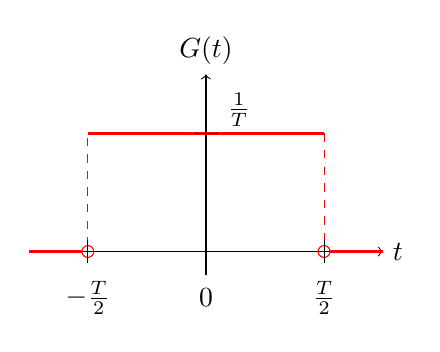
\begin{tikzpicture}[scale=1.5]
    % 绘制水平轴
    \draw[->](-1.5,0)--(1.5,0)node[right]{$t$};
    % 绘制垂直轴
    \draw[->](0,-0.2)--(0,1.5)node[above]{$G(t)$};
    % 绘制门函数
    \draw[color=red,thick](-1.5,0)--(-1.05,0);
    \draw[color=red,smooth](-1,0)circle(0.05);
    \draw[color=red,dashed](-1,0.05)--(-1,1);
    \draw[color=red,thick](-1,1)--(1,1);
    \draw[color=red,dashed](1,1)--(1,0.05);
    \draw[color=red,smooth](1,0)circle(0.05);
    \draw[color=red,thick](1.05,0)--(1.5,0);
    % 添加标签
    \draw(-1,0.1)--(-1,-0.1)node[below,outer sep=3pt]{$-\frac{T}{2}$};
    \draw(1,0.1)--(1,-0.1)node[below,outer sep=3pt]{$\frac{T}{2}$};
    \draw(0,0)--(0,0)node[below,outer sep=10pt]{$0$};
    \draw(-0.1,1)--(0.1,1)node[right]at(0.1,1.2){$\frac{1}{T}$}; 
    \end{tikzpicture}
\end{figure}
\begin{equation}
    G(t)=\left\{
        \begin{array}{cl}
        \frac{1}{T} &t\in[-\frac{T}{2},\frac{T}{2}] \\
        0 &\mbox{其他} \\
        \end{array} \right.
\end{equation} \par
\textbf{注意:}不同书籍内的门函数表达式会有所不同,但其本质不变。

\subsection{Dirac delta 函数}
\begin{equation}
    \delta(t)=\left\{
        \begin{array}{cl}
        +\infty &t=0 \\
        0 &\mbox{其他} \\
        \end{array} \right.
\end{equation} \par
并且:\par
\begin{equation}
    \int_{-\infty}^{+\infty}{\delta(\tau)\rm{d}\tau}=1
\end{equation}

\subsection{Dirac delta 函数性质}
\begin{enumerate}[align=left,label=(\arabic*)]
    \item $\int_{-\infty}^{t}{\delta(\tau)\rm{d}\tau}=\left\{
           \begin{array}{cl}
           1 &t>0 \\
           0 &t<0 \\
           \end{array} \right.$
    \item ${\delta}'(t)$ \quad ${\delta}''(t)$ \quad ${\delta}'''(t)$ \quad $\cdots$
    \item $\delta(t-t_0)=\left\{
          \begin{array}{cl}
          +\infty &t=t_0 \\
          0 &\mbox{其他} \\
          \end{array} \right.$ \quad and \quad
          $\int_{-\infty}^{+\infty}{\delta(\tau-t_0)\rm{d}\tau}=1$
    \item $A\delta(t)=\left\{
          \begin{array}{cl}
          +\infty &t=0 \\
          0 &\mbox{其他} \\
          \end{array} \right.$ \quad and \quad
          $A\int_{-\infty}^{+\infty}{\delta(\tau)\rm{d}\tau}=A$
    \item $f(t)\delta(t)=\left\{
          \begin{array}{cl}
          +\infty &t=0 \\
          0 &\mbox{其他} \\
          \end{array} \right.$ \quad and \quad
          $\int_{-\infty}^{+\infty}{f(\tau)\delta(\tau)\rm{d}\tau}=f(0)$
    \item 采样特性(sifting property):$f(t)\delta(t-t_0)=f(t_0)\delta(t-t_0)$ \quad and \par
          $\int_{-\infty}^{+\infty}{f(t)\delta(t-t_0){\rm{d}}t}=f(t_0)\int_{-\infty}^{+\infty}{\delta(t-t_0){\rm{d}}t}=f(t_0)$
    \item 对偶性:$\delta(t-t_0)=\delta(t_0-t)$ \par
          问题:$f(t)=\int_{-\infty}^{+\infty}{f(\tau)\delta(t-\tau)\rm{d}\tau}$如何推导而来?\par
          \textcircled{1} \ 令$t=\tau$,$\int_{-\infty}^{+\infty}{f(\tau)\delta(\tau-t_0)\rm{d}\tau}=f(t_0)$ \par
          \textcircled{2} \ 令$t_0=t$,$\int_{-\infty}^{+\infty}{f(\tau)\delta(\tau-t)\rm{d}\tau}=f(t)$ \par
          \textcircled{3} \ 根据性质(7),$\int_{-\infty}^{+\infty}{f(\tau)\delta(t-\tau)\rm{d}\tau}=f(t)$
    \item $[f(t)\delta(t)]'=f'(t)\delta(t)+f(t){\delta}'(t)$ \par
          $[f(t)\delta(t)]'=[f(0)\delta(t)]'=f'(0)\delta(t)+f(t){\delta}'(t)$ \par
          $f(t){\delta}'(t)=f(0){\delta}'(t)-f'(0)\delta(t)$
    \item $\int_{-\infty}^{+\infty}{f(t){\delta}'(t){\rm{d}}t}=-f'(0)$
    \item $\delta(at)=\frac{1}{|a|}\delta(t)$
\end{enumerate}

\section{卷积的性质}
\begin{enumerate}[align=left,label=(\arabic*)]
    \item 交换律:$u\ast{v}=v\ast{u}$
    \item 分配律:$(u+v)\ast{w}=u\ast{w}+v\ast{w}$
    \item 结合律:$(u\ast{v})\ast{w}=u\ast(v\ast{w})$
    \item $u(t-t_0)\ast{v(t-t_1)}=(u\ast{v})(t-t_0-t_1)$
    \item $f(t)=f(t)\ast\delta(t)$
    \item $f(t)\ast{\delta}'(t)=f'(t)\ast\delta(t)=f'(t)$
    \item $f(t)\ast{u(t)}=\int_{-\infty}^{t}{f(\tau){\rm{d}}\tau}$
    \item 如果$f_1(-\infty)=0$,$f_2(-\infty)=0$,那么$f_1(t)\ast{f_2(t)}={f_1}'(t)\ast{f_2}^{-1}(t)$
    \item $(u\ast{v})'(t)=[u(t)\ast{v(t)}]'=u'(t)\ast{v(t)}=u(t)\ast{v'(t)}$
    \item $\int_{-\infty}^{t}{[u(\tau)\ast{v(\tau)}]{\rm{d}}\tau}=\int_{-\infty}^{t}{u(\tau){\rm{d}}\tau}\ast{v(\tau)}={u(\tau)}\ast\int_{-\infty}^{t}{v(\tau){\rm{d}}\tau}$
\end{enumerate}

\section{卷积的理解}
$(f\ast{h})(t)=\int_{-\infty}^{\infty}{f(\tau)h(-\tau+t){\rm{d}}\tau}$

\end{document}